\documentclass{article}
\usepackage[top=20mm]{geometry}
\usepackage{graphicx}
\usepackage[export]{adjustbox}
\usepackage{subcaption}
\usepackage{caption}
\usepackage{multicol}


\author{Erdal Sidal Dogan \\ MEF University\\ \#041701076}
\title{MATH321 - Assignment-II}
\begin{document}
	\maketitle
	\section{Q1}
 \subsection{Q1-a}
\begin{figure}[h]
	\captionsetup[subfigure]{justification=centering}
	\begin{subfigure}[h]{0.5\textwidth}
		\hspace{2.85cm}
		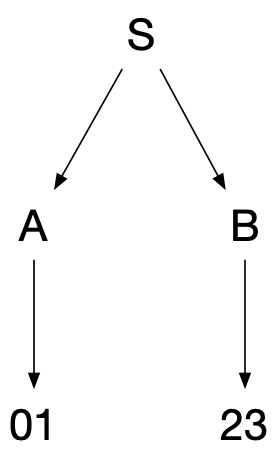
\includegraphics[scale=0.3]{Q1_a} 
		\caption{Path 1}
		\label{fig:subim1}
	\end{subfigure}
	\begin{subfigure}[h]{0.5\textwidth}
		\hspace{2.85cm}
		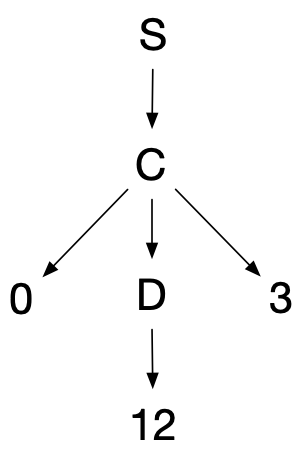
\includegraphics[scale=0.3]{Q1_b}
		\caption{Path 2}
		\label{fig:subim2}
	\end{subfigure}
	\label{fig:image2}
\end{figure}

\subsection{Q1-b}
\begin{multicols}{2}
	\noindent
	\begin{minipage}{0.5\textwidth}
		S $\rightarrow$ aABA $\mid$ aB\\
		A $\rightarrow$ bA $\mid$ b $\mid$ $ \varepsilon $\\
		B $ \rightarrow $ cB $ \mid $ c $ \mid $ $ \varepsilon $\\
		\line(1,0){150}\\
	\end{minipage}
	% \qquad
	\begin{minipage}{0.5\textwidth}
		$S_0$ $\rightarrow$ S\\
		S $\rightarrow$ aABA $\mid$ aB\\
		A $\rightarrow$ bA $\mid$ b $\mid$ $ \varepsilon $\\
		B $ \rightarrow $ cB $ \mid $ c $ \mid $ $ \varepsilon $\\
				\line(1,0){150}\\
	\end{minipage}
	% \qquad
	\begin{minipage}{0.5\textwidth}
		$S_0$ $\rightarrow$ S\\
		S $\rightarrow$ aABA $\mid$ aB $\mid$ aAA $\mid$ a\\
		A $\rightarrow$ bA $\mid$ b $\mid$ $ \varepsilon $\\
		B $ \rightarrow $ cB $ \mid $ c\\
				\line(1,0){150}\\
	\end{minipage}
	\begin{minipage}{0.5\textwidth}
		$S_0$ $\rightarrow$ S\\
		S $\rightarrow$ aABA $\mid$ aB $\mid$ aAA $\mid$ a $\mid$ aAB $\mid$ aBA $\mid$ aA\\
		A $\rightarrow$ bA $\mid$ b \\
		B $ \rightarrow $ cB $ \mid $ c \\
				\line(1,0){150}\\
	\end{minipage}
	%\qquad
	\begin{minipage}{0.5\textwidth}
		$S_0$ $\rightarrow$ S\\
		S $\rightarrow$ $A_0$ABA $\mid$ $A_0$B $\mid$ $A_0$AA $\mid$ a $\mid$ $A_0$AB $\mid$ $A_0$BA $\mid$ $A_0$A\\
		A $\rightarrow$ $B_0$A $\mid$ b \\
		B $ \rightarrow $ $C_0$B $ \mid $ c \\
		$A_0$ $ \rightarrow $ a \\
		$B_0$ $ \rightarrow $ b \\
		$C_0$ $ \rightarrow $ c \\
				\line(1,0){150}\\
	\end{minipage}
	\begin{minipage}{0.5\textwidth}
		$S_0$ $\rightarrow$ $A_{0A}B_A$ $\mid$ $A_0$B $\mid$ $A_0A_A$ $\mid$ a $\mid$ $A_0A_B$ $\mid$ $A_0B_A$ $\mid$ $A_0$A\\
		A $\rightarrow$ $B_0$A $\mid$ b \\
		B $ \rightarrow $ $C_0$B $ \mid $ c \\
		$A_0$ $ \rightarrow $ a \\
		$B_0$ $ \rightarrow $ b \\
		$C_0$ $ \rightarrow $ c \\
		$A_A$ $ \rightarrow $ AA \\
		$A_B$ $ \rightarrow $ AB \\
		$B_A$ $ \rightarrow $ BA \\
		$A_{0A}$ $ \rightarrow $ $A_0A$ \\
		
	\end{minipage}
\end{multicols}
\newpage
\subsection{Q1-c}
There must be equal number of 0's and 1's in the string. $L = \{ w \mid  w = (01)^* \cup (10)^*\}$
\section{Q2}
\begin{figure}[h]
	 \centering
	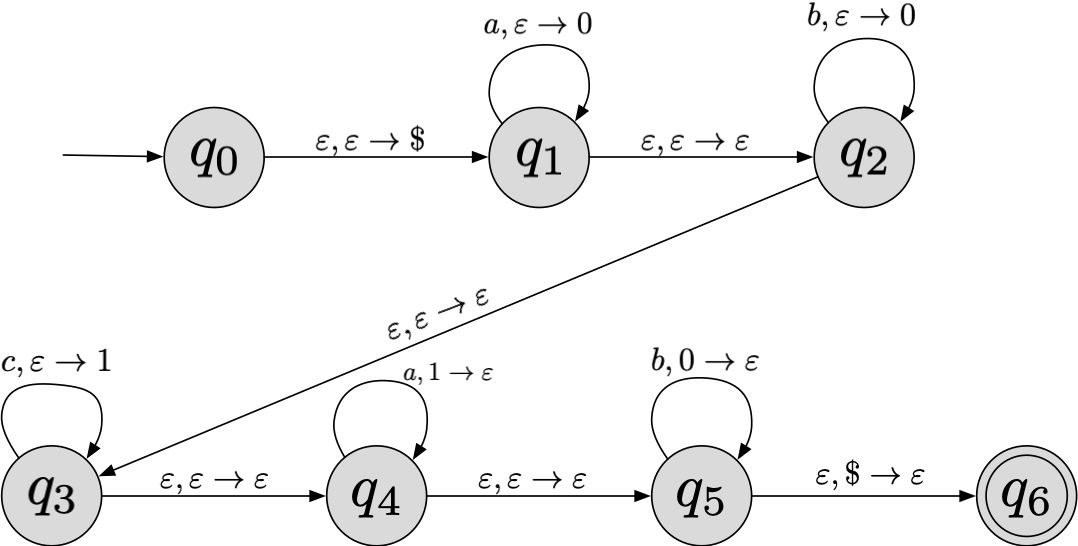
\includegraphics[scale=0.5]{Q2}
	\captionof{figure}{Push-Down Automata M}
\end{figure}
\noindent
\hspace{1.7cm} String accepted by PDA: $\varepsilon$ 	\hspace{2cm}  \qquad
String doesn't accepted by PDA: a
\begin{figure}[h]
	\captionsetup[subfigure]{justification=centering}
	\hspace{0.17\textwidth}
	\begin{subfigure}[h]{0.1\textwidth}
		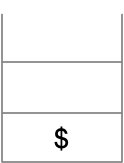
\includegraphics[scale=0.5]{Q2_epsilon}
			\caption{Initial}
	\end{subfigure}
\hspace{0.05\textwidth}
	\begin{subfigure}[h]{0.1\textwidth}
	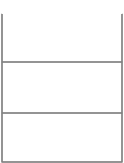
\includegraphics[scale=0.5]{Q2_epsilon_final}
	\caption{Final}
	\end{subfigure}		
	\hspace{0.23\textwidth}
	\begin{subfigure}[h]{0.1\textwidth}
		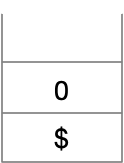
\includegraphics[scale=0.5]{Q2_a}
		\caption{Initial \& Final}
	\end{subfigure}
\end{figure}

\section{Q3}
Assume $a=b$, and pumping length $p = a = b$, then our string will be $x^{p^2}y^{p+1}x^{p+1}$\\
Break the string into $\textbf{uvxyz}$ where, $\mid \textbf{vxy} \mid \leq	p $ and $\textbf{vy} \neq \varepsilon$
\begin{itemize}
	\item \textbf{Case-I}: vxy contains only first sequence of x's;\\
	the string $uv^0xy^0z$ will contain much less number of x than $ x^{p^2} $
	
	\item \textbf{Case-II}: vxy contains both y and x;\\
	the string $uv^2xy^2z$ may satisfy the number of x or y's but the it is out of order. Consequently, not belong to the language.
	
	\item \textbf{Case-III}: vxy contains only y;\\
	the string $uv^2xy^2z$ can not contain same number of y's and trailing x's.
	
	\item \textbf{Case-IV}: vxy contains both y's and later sequence of x's;\\
	the string $uv^2xy^2z$ may satisfy the number of y and x's but the it is out of order
	
	\item \textbf{Case-V}: vxy contains only later sequence of x's;\\
	the string $uv^2xy^2z$ can not contain same number of x's and preceeding y's.
	
\end{itemize}

	
\end{document}